\documentclass[a4paper,12pt]{article}
\usepackage[left=2.5cm,right=2.5cm,top=2.5cm,bottom=2.5cm]{geometry} 
\usepackage{amsmath,amssymb,amsthm,algorithm,algorithmic,graphicx,yhmath,url,enumitem,lscape,hyperref}
\usepackage{wrapfig,subfigure}
\usepackage{lineno}

\newcounter{problem}
\newcounter{remark}
\newcounter{hint}
\newenvironment{remark}{\refstepcounter{remark} \vspace{0.1cm} \par \noindent {\bf Remark \arabic{remark}}}{\vspace{0.3cm}}
\newenvironment{hint}{\refstepcounter{hint} \vspace{0.1cm} \par \noindent {\bf Hint \arabic{hint}}}{\vspace{0.3cm}}
\newcommand{\R}{\mathbb{R}}
\newcommand{\N}{\mathbb{N}}
\newcommand{\Rn}{\mathbb{R}^n}
\newcommand{\Rnn}{\mathbb{R}^{n \times n}}
\newcommand{\bes}{\begin{equation*}}
\newcommand{\ees}{\end{equation*}}
\newcommand{\be}{\begin{equation}}
\newcommand{\ee}{\end{equation}}
\newcommand{\bms}{\begin{multline*}}
\newcommand{\emults}{\end{multline*}}

% Matrices
\newcommand{\bbm}{\begin{bmatrix}}
\newcommand{\ebm}{\end{bmatrix}}
\newcommand{\bpm}{\begin{pmatrix}}
\newcommand{\epm}{\end{pmatrix}}

% Strecthing
\renewcommand{\arraystretch}{1.3}

\newcommand{\eps}{\epsilon}
\newcommand{\fl}{\text{fl}}
\newcommand{\Lp}{{L^p}}
\newcommand{\Ker}{\text{Ker}\,}
\newcommand{\loc}{{\text{loc}}}
\newcommand{\ccinf}{C_c^\infty}
\newcommand{\supp}{\text{supp}}
\newcommand{\dist}{\text{dist}}

% Gravitational acceleration
\newcommand{\bg}{\mathbf{g}}
% Friction force
\newcommand{\bFf}{\mathbf{F_f}}
% Gravitational force
\newcommand{\bFg}{\mathbf{F_g}}
% Force
\newcommand{\bF}{\mathbf{F}}
% Position, velocity, acceleration
\newcommand{\br}{\mathbf{r}}
\newcommand{\bv}{\mathbf{v}}
\newcommand{\ba}{\mathbf{a}}

% Jacobian
\newcommand{\bDF}{\mathbf{DF}}

\newtheorem{theorem}{Theorem}[section]
\newtheorem{proposition}[theorem]{Proposition}
\newtheorem{lemma}[theorem]{Lemma}
\newtheorem{definition}[theorem]{Definition}
\title{Approximation of real functions and solution of non-trivial equations}
\author{Carl Christian Kjelgaard Mikkelsen}

\begin{document} 

\pagenumbering{arabic}
% Turn off line numbering by commenting the following line.
% \linenumbers
\thispagestyle{empty}

\noindent
Ume\aa{} University \hfill Fall 2018 \\
Department of Computing Science\\

\vskip 2.5cm

\begin{center} {\Huge {\bf Project 2}}\\{\Large Approximation of real functions and solution of non-trivial equations}\end{center} \vskip 0.3cm
\begin{center}
  {\huge Scientific Computing}
  \vfill
  {\Large The deadline for this project can be found at: \href{http://www8.cs.umu.se/kurser/5DV005/HT18/planering.html}{http://www8.cs.umu.se/kurser/5DV005/HT18/planering.html}\\
  (Link \emph{Overview} on the course homepage.)}
\end{center}
  \vfill
  {% \large
\begin{itemize}
\item The submission should consist of:
  \begin{itemize}
  \item The complete report, including
    \begin{itemize}
    \item A front page with the following information:
      \begin{enumerate}
      \item Your {\bf name}.
      \item The {\bf course name}.
      \item Your {\bf username} at the Department of Computing
        Science.
      \item The {\bf project number}.
      \item The {\bf version} of the submission (in case of re-submissions).
      \end{enumerate}
    \end{itemize}
  \item An appendix with the source code.
  \item To simplify feedback, the main report (optionally excluding
    the appendix) must have {\bf numbered sections} and {\bf page
      numbers}.
  \end{itemize}
\item The submitted code must be Matlab-compatible. If you choose to
  work in Octave, verify that your code is Matlab-compatible before
  you submit your project.
\item If you write your report using \LaTeX, double-check that your
  references have been resolved correctly before you submit. ``Figure ??'' is useless to any reader.
\item Your report should be submitted as a pdf file uploaded via
  the\linebreak 
  \href{https://webapps.cs.umu.se/labresults/v2/handin.php?courseid=337}{https://webapps.cs.umu.se/labresults/v2/handin.php?courseid=337}
  page, also available as the
\begin{center}
  \href{http://www8.cs.umu.se/kurser/5DV005/HT18/index2.html}{Submit/Check results}
\end{center} link at the bottom left of the course home page.
\item Furthermore, every scrap of MATLAB code developed by your team should be uploaded in a single zip file, {\tt P1Code.zip}.
\end{itemize}
  }
  \vfill

\newpage

\maketitle

\tableofcontents
\listoffigures

\section{Purpose} Let $I = [a,b] \subset \R$ and let $f: I \rightarrow \R$ denote a function. In this project we consider the problem of computing $f$ and solving the equation $f(x) = 0$. Frequently, but not universally, our knowledge of $f$ is limited to a table of function values, say, 
\bes
\begin{array}{|c|c|c|c|c|} \hline
  x_0 & x_1 & x_2 & \dots & x_n \\ \hline
  f(x_0) & f(x_1) & f(x_2) & \dots & f(x_n) \\ \hline
\end{array}
\ees
We must construct accurate approximations of $f(t)$ for all $t \in [x_0,x_n]$ from this data. You will develop software which can compute accurate approximations and solve complicated equations accurately.
  
\section{The zero theorems} Much our work hinges on a set of theorems which assert the existence of a zero:
  \begin{itemize}
  \item Robust root finding for a continuous function $f : I \rightarrow \R$ requires a bracket $(a_0,b_0)$ such that $f(a_0)f(b_0) < 0$. By the intermediate value theorem there exists at least one zero $r \in (a_0,b_0)$.
  \item If $a_0 \in I$ and $b_0 \in I$ are zeros of a differentiable function $f : I \rightarrow \R$, then by Rolle's theorem. there exists $c$ between $a_0$ and $b_0$ such that
    \bes f'(c)=0.
    \ees
  \item  If $a_0 \in I$ and $b_0 \in I$ and $f : I \rightarrow \R$, is differentiable, then by the mean value theorem there exists $c$ between $a_0$ and $b_0$ such that
    \be
    f'(c)=\frac{f(b)-f(a)}{b-a}
    \ee
  \end{itemize}

  Assignment 1 ruthlessly exploited the intermediate value theorem. You will now develop a scripts which illustrates both Rolle's theorem and the mean value theorem.

  \begin{enumerate} \item
    Copy {\tt a2f1.m} into {\tt no2/work/MyZeroTheorem.m} and complete the script according to the specifications. The script is finished when it reproduces Figure~\ref{fig:MyZeroTheorems}.
  \end{enumerate}

  \begin{figure}
    \centering
    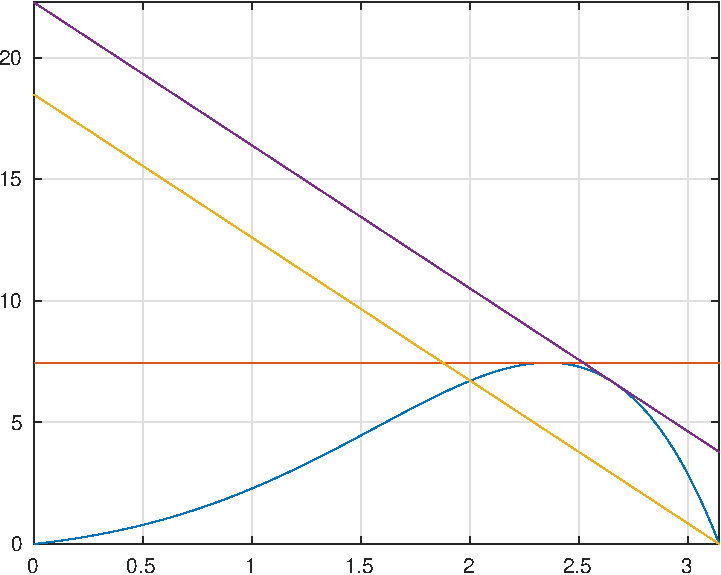
\includegraphics[width=10cm]{MyZeroTheorems.pdf} \caption[Illustration of central theorems]{A illustration of Rolle's theorem and the mean value theorem of differentiation.} \label{fig:MyZeroTheorems}
    \end{figure}

  
  \section{Approximation of derivatives}

  Let $f : I \rightarrow \R$ be a function which is infinitely often differentiable. Let $h > 0$. By Taylor's theorem we have
  \bes
  f(x + h) = f(x) + f'(x) h + \frac{1}{2} f''(x) h^2 + \dotsc, \frac{1}{p!} f^{(p)}(x) h^p + O(h^{p+1}), \quad h \rightarrow 0, \quad h > 0.
  \ees
  \begin{enumerate}
  \item Show that
    \be \label{equ:space-central}
    f'(x) = \frac{f(x+h) - f(x-h)}{2h} + O(h^2), \quad h \rightarrow 0, \quad h > 0.
    \ee
  \item Show that
    \be \label{equ:left-endpoint}
    f'(x) = \frac{-3 f(x) + 4 f(x+h) - f(x+2h)}{2h} + O(h^2), \quad  h \rightarrow 0, \quad h > 0.
    \ee
  \item Show that 
    \be \label{equ:right-endpoint}
    f'(x) = \frac{f(x-2h)-4f(x-h)+3f(x)}{2h} + O(h^2), \quad  h \rightarrow 0, \quad h > 0.
    \ee
  \item Copy {\tt a2f2.m} into {\tt no2/work/MyDerivs.m} and complete the function according to the specification. It likely that {\tt MyDerivs} is working correctly when the minimal working example {\tt a2f3.m} regenerates Figure~\ref{fig:MyDerivs}.
  \item What evidence do you find to support the hypothesis that error committed by {\tt MyDerivs} is $O(h^2)$ as suggested by equations \eqref{equ:space-central}, \eqref{equ:left-endpoint}, \eqref{equ:right-endpoint}?
 \end{enumerate}

 \begin{figure}
    \centering
    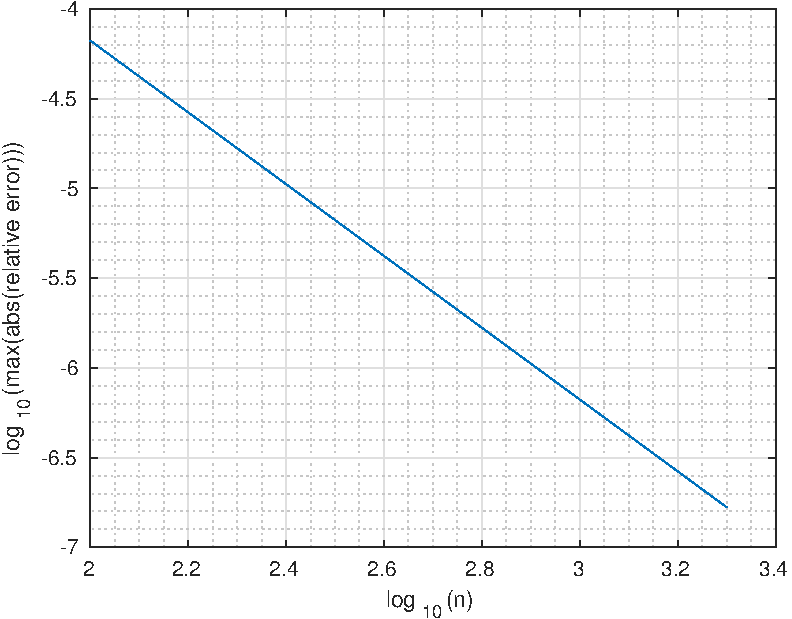
\includegraphics[width=10cm]{MyDerivs.pdf} \caption[The error of finite difference approximations of the derivative]{The error of finite difference approximations of the first derivative decay rapidly when decreasing the stepsize $h$ between the sample points.} \label{fig:MyDerivs}
    \end{figure}

 
 \section{Hermite's piece-wise approximation}
 Consider the polynomials $p_0$, and $p_1$ given by
 \be
 p_0(t) = (1 + 2t)(1-t)^2, \qquad  p_1(t) = t^2 (3-2t) \\
 \ee
 as well as the polynomials $q_0$ and $q_1$ given by
 \be
 q_0(t) = t(1-t)^2, \qquad q_1(t) = t^2 (t-1).
 \ee
   
 \begin{enumerate}
 \item Show that
   \be
   p_0(0) = 1, \quad p_0(1) = 0, \quad p_0'(0) = 0, \quad p_0'(1) = 0.
   \ee
 \item Show that
   \be
   p_1(0) = 0, \quad p_1(1) = 1, \quad p_1'(0) = 0, \quad p_1'(1) = 0.
   \ee
  \item Show that
   \be
   q_0(0) = 0, \quad q_0(1) = 0, \quad q_0'(0) = 1, \quad q_0'(1) = 0.
   \ee
 \item Show that
   \be
   q_1(0) = 0, \quad q_1(1) = 0, \quad q_1'(0) = 0, \quad q_1'(1) = 1.
   \ee
 \end{enumerate}
 Consider a function $f : [a,b] \rightarrow \R$ such that $f$ is differentiable and $f'$ is continuous. Let $\phi : [a,b] \rightarrow \R$ denote the linear function which maps $a$ into $0$ and $b$ into $1$, i.e.,
 \be
 \phi(x) = \frac{x - a}{b-a}.
 \ee
 Hermite's approximation of $f : [a,b] \rightarrow \R$ is the polynomial $p : [a,b] \rightarrow \R$ given by
 \be
 p(x)  = f(a) p_0(\phi(x)) + f(b) p_1(\phi(x)) + f'(a) (b-a) q_0(\phi(x)) + f'(b) (b-a) q_1(\phi(x))
 \ee
 \begin{enumerate}[resume]
 \item Show that Hermite's approximation satisfies
   \be
   p(a) = f(a), \quad p(b) = f(b), \quad p'(a) = f'(a), \quad p'(b) = f'(b).
   \ee
 \end{enumerate}
 In short, Hermite's approximation reproduces the values of $f$ and $f'$ at the endpoints of the intervals. If we are given a list of points
 \bes
 a= x_0 < x_1 < x_2 < \dots < x_n = b
 \ees
 as well as the function values $f(x_j)$ and the derivatives $f'(x_j)$, then we can approximate $f$ using a piece-wise cubic polynomial $p : [a,b] \rightarrow \R$ given by
 \be
\forall x \in [x_{j-1},x_j] \: : \: p(x) = p_j(x)
 \ee
 where $p_j$ is Hermite's approximation of $f$ corresponding to the sub-interval $[x_{j-1}, x_j]$. By design, the function $p$ is differentiable and $p'$ is continuous.
\begin{enumerate}[resume] 
 \item Copy {\tt a2f4.m} into {\tt no2/work/MyPiecewiseHermite} and complete the function according to the specification. It is likely that {\tt MyPiecewiseHermite} is working correctly when the minimal working example {\tt a2f5.m} generates Figure~\ref{fig:MyPiecewiseHermite}.

 \item What evidence do you find to support the conjecture that the error $f(x) - p(x)$ decays as $O(h^4)$?
 \end{enumerate}

 \begin{figure}
    \centering
    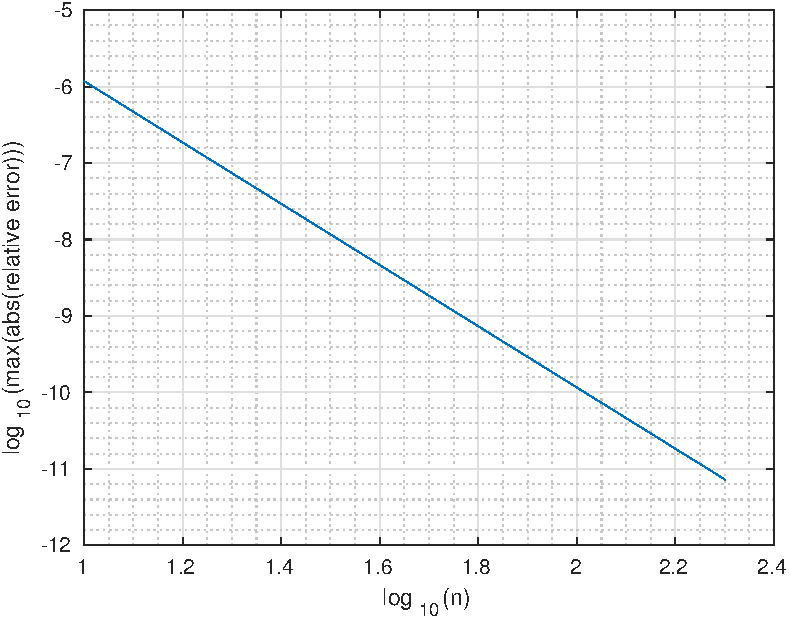
\includegraphics[width=10cm]{MyPiecewiseHermite.pdf} \caption[The error of the piecewise Hermite approximation]{The error of a piecewise Hermite approximation decays rapidly when we decrease the stepsize $h$ between the sample points.} \label{fig:MyPiecewiseHermite}
    \end{figure}

 
   \section{Event location for ordinary differential equations}

   The function {\tt range\_rkx} computes the position $(x(t),y(t))$ and velocity $(x'(t),y'(t))$ of an artillery shell by solving an ordinary differential equation
   \bes
   \gamma'(t) = f(t,\gamma(t)
   \ees
   with respect to the function $t \rightarrow \gamma(t)$ which satisfies
   \bes
   \gamma(t) = (x(t), y(t), x'(t), y'(t))^T.
   \ees
   The specific function $f$ is complicated and describes all the necessary physics. In practice, we are not particularly interested in the trajectory itself, rather we seek to solve nonlinear equation of the form
   \bes
   g(\gamma(t)) = 0,
   \ees
   where $g$ is a function such that the composition $g \circ \gamma$ is defined. For the sake of simplicity, we assume that $g$ is defined for all $z \in \R^4$, and write
   \bes
   g(z) = g(z_1, z_2, z_3, z_4).
   \ees
   The function $g$ is called an event function and we say that an event has occurred at time $t$ if $g(\gamma(t)) = 0$. Obviously, some events function are more interesting than others.
   
   \begin{itemize}
   \item The choice of $g(z) = z_2 - c$ corresponds to solving the nonlinear equation
     \be
     y(t) = c
     \ee
     This is equivalent to finding the time $t$ where the shell reaches the height $c$. 
   \item If $x \rightarrow h(x)$ is a function which represents the height of the landscape, then the choice of $g(z) = z_2 - h(z_1)$ corresponds to solving the nonlinear equation
     \bes
     y(t) - h(x(t)) = 0.
     \ees
     This is equivalent to computing the time $t$ where the shell hits the ground.
   \end{itemize}
   By necessity, we are limited to computing a \textit{finite} set of approximations, say, $\gamma(t_j)$ for $j=0,1,\dots,m$. However, the use of Hermite's approximations allows us to extend our approximation to cover the entire interval $[t_0,t_m]$. This allows us to rapidly \textit{approximate} the solution(s) of an event equation.

   \begin{enumerate}
   \item Copy the minimal working example {\tt range\_rkx\_mwe1} into the file {\tt no2/work/MyEvent.m}. Extend {\tt MyEvent} to the point where it defines Hermite's approximation of both $t \rightarrow x(t)$ and $t \rightarrow y(t)$ and solves the non-linear equation $y(t) - h(x(t)) = 0$ where $x \rightarrow h(x) $ is the small hill defined by the script {\tt a2f6.m}, see Figure~\ref{fig:MyEvent}.
   \end{enumerate}

\begin{figure}
    \centering
    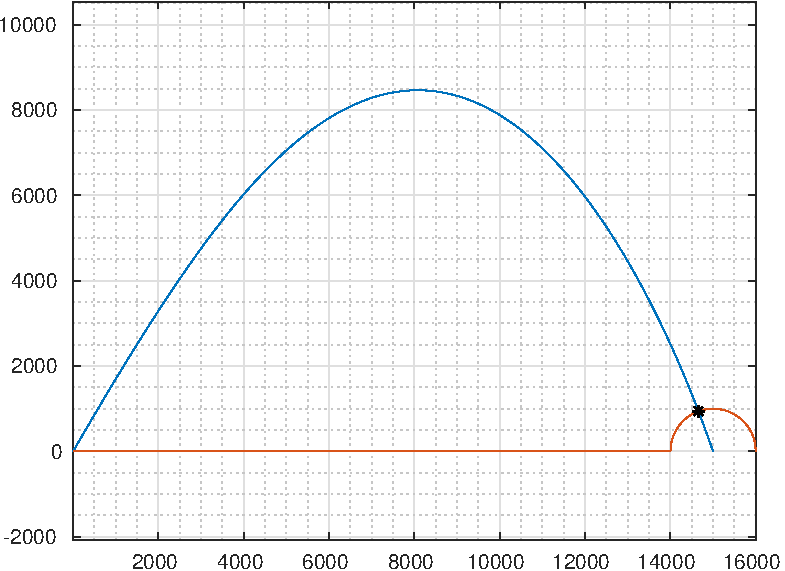
\includegraphics[width=10cm]{MyEvent.pdf} \caption[The point of impact between a shell and a simple landscape]{The point of impact between a shell and a simple landscape, i.e. a spherical hill.} \label{fig:MyEvent}
    \end{figure}

    \begin{remark} The computed solution of an event equation depends on the size of the time step used to approximate the trajectory in the first place. Estimating the error, i.e. the difference betweeen the computed solution and the real solution is a non-trival problem. It will take us a few weeks to develop the necessary skills.
   \end{remark}

   
   \bibliographystyle{plain}
\bibliography{../../../lecture-notes/refs}


  
\end{document}

